\section{Equações diferenciais}
Boa parte do que se faz em ciência e tecnologia envolve fenômenos cujas equações básicas são conhecidas mesmo que se saiba pouco sobre o fenômeno em si. Tomemos como exemplo o escoamento de um fluido Newtoniano incompressível ao redor de um cilindro de grande comprimento. As equações básicas, equações de Navier-Stokes são conhecidas a quase 2 séculos mas este continua sendo um problema onde ocorre muita pesquisa, com muitos artigos em revistas científicas e pesquisadores ao redor do mundo empenhando grandes esforços neste problema aparentemente simples. Esta é uma situação comum em ciência. 

O fato de se conhecer os princípios básicos e as respectivas equações não quer dizer que o problema está resolvido. Mas é importante lembrar que estas equações continuam válidas mesmo que alguns detalhes do problema sejam nebulosos. Nesta seção, alguns problemas (modelos) serão analisados a partir de suas equações básicas.

\subsection{Pêndulo simples}

\begin{figure}
\centering
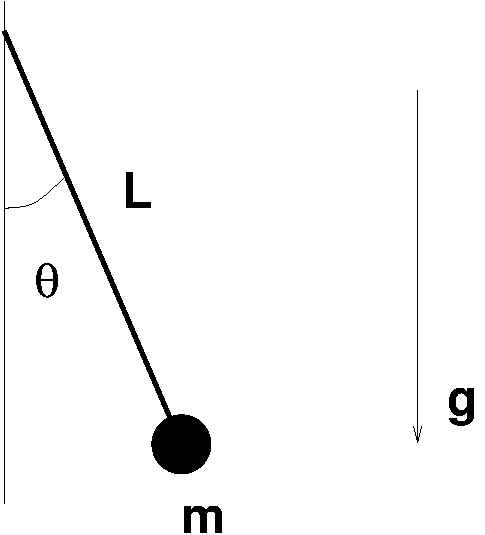
\includegraphics[width=0.4\textwidth]{./figuras/pendulo.pdf}
\vspace{0.5cm}
\caption{Pêndulo simples}
\label{fig:pendulo}
\end{figure}

O pêndulo simples é um dos problemas mais conhecidos na física básica. A figura \ref{fig:pendulo} mostra um diagrama esquemático do pêndulo simples. A palavra ``simples'' deve ser enfatizada. Este problema introdutório em cursos de físicas é uma idealização do problema real. Nesta idealização, os únicos parâmetros importantes são a massa do pêndulo, que neste modelo idealizado some, a aceleração da gravidade, que é constante, o comprimento do pêndulo e o ângulo inicial em que se solta o pêndulo. Nesta idealização, a dimensão da massa é desprezada e a única caractérística do fio é o seu comprimento que é constante. Efeitos como resitência do ar, elasticidade do fio, rotação da terra são desprezados. Se levados em conta, o problema é consideravelmente mais complexo. 

\subsubsection{O que se pode desprezar}
Mas não é tudo, outros fatores influenciam este problema como, por exemplo, a variação de $\textbf{g}$ com a posição. No limite, até a dinâmica dos átomos do ar e a radiação solar incidente interferem. Levando em conta tudo este problema não seria resolvido. Neste sentido, o mais importante é saber o que ignorar. Apenas os efeitos com as escalas corretas. Imaginemos que este pêndulo é uma esfera de aço com 1 cm de diâmetro. Se esta esfera refletir toda a luz incidente, a razão entre a força gerada pela pressão da luz do sol na terra e a força da gravidade vale (ordem de grandeza):
\[
\frac{F_{sol}}{F_{grav}} \approx \frac{W''}{\rho D g c} \approx 5\times 10^{-9}
\]
onde $W''=1360\:W/m^2$ é o fluxo de radiação solar. Com valores baixos como este, á fácil desprezar o efeito da radiação solar. 

Por outro lado, se o pêndulo tiver velocidade típica da esfera for de 1 m/s e estiver no ar, a razão entre a força peso e a força de arrasto aerodinâmica vale:
\[
\frac{F_{aero}}{F_{grav}} = \frac{3\cdot C_D \rho_a V^2}{32\cdot\rho D g} \approx 0,02\%
\]

Este valor de 0,02\% é pequeno mas seu efeito acumulado pode ser considerável (pêndulos param) e dependendo do que se deseja, deve ser incluido. No entanto, é importante observar que, por este valor ser pequeno, um modelo simples com incerteza alta para a força de arrasto geralmente é suficiente para a maioria dos problemas. Caso contrário teria que se resolver o problema do escoamento ao redor da esfera, o que, como será visto adiante, não é um problema simples.

\subsubsection{Modelo matemático simples}
Com todas as simplificações anteriores, chega-se à equação do pêndulo simples:

\[
m\cdot L^2\cdot\frac{d^2\theta}{dt^2} + m\cdot g\cdot L\cdot \sin\theta = 0
\]
com as seguintes condições de contorno:
\[
t = 0 \qrq \theta=\theta_0, \quad\frac{d\theta}{dt} = 0
\]

Esta equação pode ser reescrita como:
\[
\frac{L}{g}\frac{d^2\theta}{dt^2} + \sin\theta = 0 
\]
Definindo 
\[
t_* = \frac{t}{t_0}\qrq \quad\text{onde}\quad t_0 = \sqrt{\frac{L}{g}}
\]
chega-se à equação adimensional
\[
\frac{d^2\theta}{dt_*^2} + \sin\theta = 0 
\]

Agora, sabendo $\theta_0$ (condição de contorno inicial) resolvendo esta equação, está se resolvendo qualquer pêndulo simples. Quando $\theta_0$ é pequeno, $\sin\theta_0\approx\theta_0$ e a equação diferencial é linearizada. Sua solução é simples e o período do pêndulo vale:
\[
T = 2\pi\sqrt{\frac{L}{g}}
\]
Partindo desta solução aproximada pode-se obter uma expressão para o problema não linear utilizando métodos assintóticos:
\[
T = 2\pi\sqrt{\frac{L}{g}}\cdot\varphi(\theta_0) = 2\pi \sqrt{\frac{L}{g}} \cdot\left[\varphi(0) + \theta_0\cdot\varphi'(0) +
\frac{1}{2}\theta_0^2\cdot\varphi'' + \ldots\right]
\]
o que se observa neste problema simples é que a formulação do problema simplificado (idealizado) exige a desprezar diferentes fenômenos físicos. Para tanto é necessário achar estimativas, mesmo que grosseiras, das diferentes influências. Uma vez que se simplificou o problema, pode-se fazer mais, utilizando análise dimensional, o que consiste basicamente em reescalar o problema. Neste ponto maiores simplificações são, algumas vezes, possíveis.

Uma outra maneira se enxergar este processo (análise dimensional) é considerar que pode-se escolher um outro sistema de unidades onde os coeficientes (neste caso $\sqrt{L/g}$) valem 1.

\subsection{Difusão de calor}
\subsubsection{Problema 3D}
Neste caso, o problema é modelado por uma equação diferencial parcial. Vale ressaltar que para se chegar a esta equação diferencial, o problema já foi simplificado. O problema da difusão de calor linear é modelado pela seguinte equação diferencial:
\[
\frac{\partial u}{\partial t} = \alpha\nabla^2 u
\]
onde $u$ é a temperatura e $\alpha$ é o coeficiente de difusão de calor do material. Além disso, ainda faltam as condições de contorno. Quando o domínio é um cubo de lado $L$ formado pelas faces $x=0,L$m $y=0,L$ e $z=0,L$ e as condições de contorno forem $u=0$ na face $x=0$, $u=u_0$ e nas demais o fluxo de calor é nulo, ou seja, a derivada da temperatura em relação à normal da face é zero. A condição inicial é $u=0$. O objetivo deste problema é obter $u(x,y,z,t)$ para $t>0$:
\[
u = f(u_0, L, \alpha, x, y, z, t)
\]
A equação fornece uma escala de dimensão $L$ e escala de temperatura $u_0$. Estas escalas permitem definir novos parâmetros que na região de interesse possuem valores da ordem de 1: $x_* = x\cdot L$, $y_* = y\cdot L$, $z_* = z\cdot L$, e $u_* = u\cdot u_0$. Dentro do cubo, tanto as coordenadas $(x_*, y_*, z_*)$ quanto a temperatura $u_*$  possuem valores entre 0 e 1. Substituindo estas relações na equação diferencial temos:
\[
\frac{\pd u_*}{\pd t} = \frac{\alpha}{L^2}\left(\frac{\pd^2 u_*}{\pd x_*^2} + \frac{\pd^2 u_*}{\pd y_*^2} + \frac{\pd^2 u_*}{\pd z_*^2} \right) = \frac{\alpha}{L^2} \nabla_* u_*
\]
Esta equação sugere uma escala de tempo: $t = t_*\cdot t_0 = t_* \cdot \frac{L^2}{\alpha}$. Substituindo esta relação na equação anterior chega-se à seguinte relação:
\[
\frac{\pd u_*}{\pd t_*} =\nabla_* u_*
\]
As condições de contorno são $u_*=0$ em $x_*=0$, $u_*=1$ em $x_*=1$ e nas demais faces o fluxo é zero: $\pd u_*/\pd y_* = 0$ em $z_*=0,1$ e $\pd u_*/\pd z_* = 0$ em em $y_*=0,1$.


As condições de contorno também se simplificam: $u_*=0$ em $x_*=0$, $y_*=0$, $z_*=0$, $y_*=1$, $z_*=1$ e $u_* = 1$ em $x_* = 1$. 

A solução deste novo problema é:
\[
u = u_0 \cdot \varphi(t_*, x_*, y_*, z_*) = u_0\cdot\varphi\left(\frac{t\alpha}{L^2}, \frac{x}{L}, 
 \frac{y}{L} , \frac{z}{L}\right)
\]
O problema original tinha 7 parâmetros e foi reduzido para 4, o que é um ganho substancial. Novamente, para este tipo de geometria e este tipo de condição de contorno, a solução deste problema adimensional vale para quaisquer valores de $L$, $\alpha$ e $u_0$. Outro aspecto interessante é que no domínio/tempo de interesse, todos os parâmetros são da ordem um, $\mathcal{O}(1)$.

\subsubsection{Uma barra fina e comprida}

Modificando o problema de modo que o domínio é um paralelepípedo com lados $L_x=L$, $L_y$ e $L_z$, onde $L \gg L_x$ e $L \gg L_y$, as variações da temperatura nas direções $y$ e $z$ para $x$ constante são desprezíveis e portanto a equação diferencial pode ser simplificada de modo que 
\[
u(x, y, z, t) = u(x, t)
\]
e portanto

\[
\frac{\pd u}{\pd t} = \alpha \frac{\pd^2 u}{\pd x^2}
\]
Como na subseção anterior, chega-se a uma equação adimensional. Repetindo o procedimento da seção anterior, chega-se à seguinte equação adimensional:
\[
\frac{\pd u_*}{\pd t_*} = \frac{\pd^2 u_*}{\pd x_*^2} \qrq u = u_0\cdot\varphi\left(\frac{t\alpha}{L^2}, \frac{x}{L}\right)
\]
A solução deste problema com $t\lra\infty$ é a velha distribuição linear de temperatura:
\[
u(x,\infty) \lra \frac{x}{L}\cdot u_0
\]
Mas nos outros instantes de tempo é necessário resolver a equação acima. Outras simplificações são possíveis quando $L$ é muito grande ou quando $t$ é muito pequeno.

\subsubsection{Auto-semelhança: barra infinita}
O que acontece se a barra for muito comprida (ou o logo no começo)? Neste caso, não existe uma escala de comprimento pré-definida. Assim esta escala deve sair do próprio problema. Ou seja, se $L\lra\infty$, para que o tempo adimensional seja constante:
\[
\frac{t\alpha}{L^2} = cte \qrq L = \sqrt{t\alpha} \qrq \eta = \frac{x}{L} = \frac{x}{\sqrt{\alpha t}} \qrq \frac{u}{u_0} = f(\eta)
\]
Usando esta escala na equação diferencial parcial, chega-se à seguinte equação diferencial \emph{ordinária}:
\[
f''(\eta) + \frac{\eta}{2} f'(\eta) = 0
\]
com condições de contorno
\[
f(0) = 0 \qquad\qquad \lim_{\eta\lra\infty} f(\eta) = 1
\]
Com esta mudança de variáveis, transformou-se uma equação diferencial parcial em uma equação diferencial ordinária, algo que é significativo. Neste caso, a solução analítica desta equação é simples:
\[
f(\eta) = \mathrm{erf}\left(\frac{\eta}{2}\right)
\]
onde $\mathrm{erf}$ é a função erro.

\section{Escoamento incompressível ao redor de uma esfera}


Os examplos anteriores usaram modelos simples e/ou lineares para mostrar como as principais escalas de um problema permitem simplificar equações diferenciais. Nesta seção será analisado o escoamento ao redor de uma esfera. Admitindo um fluido newtoniano incompressível, chega-se às equações de Navier-Stokes:

\begin{equation}
\frac{\pd\p{u}}{\pd t} + \p{u}\cdot\nabla\p{u} = -\frac{1}{\rho}\nabla p + \nu\nabla^2\p{u} \qquad\qquad \nabla\cdot\p{u} = 0
\label{eq:ns}
\end{equation}
onde $\p{u}$ é o vetor velocidade, $p$ é o campo de pressões, $\nu$ é a viscosidade cinemática e $\rho$ é a densidade do fluido. O problema do escoamento ao redor de uma esfera em um ambiente grande apresenta as seguintes condições de contorno:
\[
 r\lra\infty \quad \p{u}\lra U_0\p{\hat{i}} \qquad\qquad r=\frac{D}{2}\quad \p{u} = \p{0}
\]
a segunda condição anterior corresponde à aderência do fluido na parede da esfera. Estas condições de contorno fornecem uma escala para a velocidade $U_0$ e uma escala para a dimensão $D$ (o diâmetro da esfera). Seguindo o mesmo procedimento adotado para o problema de difusão, obtém-se os seguintes parâmetros para o problema:

\[
\begin{aligned}
&x_* = \frac{x}{D}, \quad y_* = \frac{y}{D}, \quad z_* = \frac{z}{D}\\
&\p{u}_* = \frac{\p{u}}{U_0}, \quad p_* = \frac{p}{P_0}, \quad t_* = \frac{t}{t_0} = \frac{tU_0}{D} \\
\end{aligned}
\]
Observe que o parâmetro $P_0$ ainda é desconhecido e será analisado mais adiante. Antes, porém, é interessante notar que não existe uma equação para a pressão e ela não aparece nas condições de contorno. Na verdade, a pressão ela aparece como resultado das equações de Navier-Stokes e seu valor é tal que a equação da continuidade ($\nabla\cdot\p{u}=0$) é satisfeita. Usando as escalas corretas os parâmetros anteriores possuem valores com ordem de grandeza $\mathcal{O}(1)$. Isto pode parecer estranho a primeira vista já que o domínio se estendo ao infinito. No entanto as coisas mais relevantes acontecem perto da esfera. É neste sentido que $x_*, y_*, z_* \sim 1$. Um argumento semelhante pode ser utilizado para o tempo $t_*$. É lógico que o escoamento pode durar um intervalo de tempo grande (uma bola pode ficar durante dias dentro de um túnel de vento) mas o tempo que leva para uma partícula passar por perto da esfera corresponde a  $t_*\sim 1$. 

Com estes novos parâmetros, chega-se às equações de Navier-Stokes adimensionais:

\begin{equation}
\frac{\pd\p{u}_*}{\pd t_*} + \p{u}_*\cdot\nabla_*\p{u_*} = -\frac{P_0}{\rho U_0^2}\nabla_* p_* + \frac{1}{Re}\nabla_*^2\p{u}_* \qquad \nabla_*\cdot\p{u}_* = 0
\label{eq:ans}
\end{equation}
nestas equações, $Re = \frac{U_0 D}{\nu}$ é o número de Reynolds e 
\[
\nabla_* = \frac{\pd}{\pd x_*} \p{\hat{i}} + \frac{\pd}{\pd y_*} \p{\hat{j}} + \frac{\pd}{\pd z_*} \p{\hat{k}}
\]
e as condições de contorno são:
\[
 r_*\lra\infty \quad \p{u}_*\lra \p{\hat{i}} \qquad\qquad r_*=\frac{1}{2}, \p{u}_* = \p{0}
\]

Como se observou para o pêndulo simples e a difusão de calor, introduzir as escalas principais do problema reduz o trabalho significativamente se originalmente
\[
u = f(t, x, y, z, U_0, D, \nu, \rho)
\]
Com esta análise dimensional, o problema se reduziu a 
\[
u = U_0 \varphi\left(\frac{t U_0}{D}, \frac{x}{D}, \frac{y}{D}, \frac{z}{D}, \frac{U_0 D}{\nu}\right)
\]

Se antes, além do tempo e coordenadas,  eram  necessários resolver o problema para quatro parâmetros independentes ($U_0$, $D$, $\nu$ e $\rho$), agora, apenas o número de Reynolds é necessário. A economia de esforços é considerável, assim como a liberdade que se ganha: experimentos podem ser realizados em diferentes fluidos se $Re$ for o mesmo.

Este resultado ó obtido na análise dimensional tradicional. No entanto é interessante lembrar que nesta formulação, cada termo $u_*$ tem ordem de grandeza 1 por construção e aparecem dentro de derivadas. Dependendo das circunstâncias, estimativas relativas de cada termo desta equação podem ser feitas de modo a desprezar alguns termos e simplificar o problema.

\subsection{Equações de Euler - $Re\lra\infty$}

Uma aproximação de \ref{eq:ans} que salta à vista é o limite 
\[
Re \lra\infty
\]
Se admitirmos que o escoamento está em regime permanente (RP), $\pd/\pd t = 0$, obtém-se as equações de Euler:

\begin{equation}
\p{u}_*\cdot\nabla_*\p{u_*} = -\frac{P_0}{\rho U_0^2}\nabla_* p_* %\qqrq P_0\sim\rho U_0^2
\label{eq:euler}
\end{equation}
por construção, o lado esquerdo desta equação tem ordem de grandeza 1. Para que o gradiente de pressão tenha, também, ordem de grandeza 1, é basta definir  
\[
P_0 = \rho U_0^2
\]

A equação de Euler ainda possue o termo convectivo não linear mas já não é uma equação de segunda ordem. Isto tem consequências, principalmente perto da parede pois nas equações de Euler, a velocidade junto a parede não é nula. Mas longe da parede as equações de Euler podem ser representativas, principalmente se não houver separação.

\subsection{Equação de Stokes}
Um outro limite é quando $Re\lra 0$. Neste caso não faz sentido empregar $P_0 = \rho U_0^2$ que foi obtido admitindo $Re$ grande. Novamente, considerando o escoamento em regime permanente e multiplicando ambos os lados da equação por $Re$, 
\[
Re\left(\p{u}_*\cdot\nabla_*\p{u_*}\right) = -Re\frac{P_0}{\rho U_0^2}\nabla_* p_* + \nabla_*^2\p{u}_* \qquad\qquad \nabla_*\p{u}_* = 0
\]
por construção, o termo convectivo tem ordem 1 e  vai para zero. Infelizmente não se pode simplesmente desprezar o termo da pressão. Fazendo $Re$ tender a zero mantendo $D$, $\rho$ e $\nu$ fixos, o denominador $\rho U_0^2$ vai para zero mais rapidamente que $Re$ que está no numerador e portanto este termo não pode ser desprezado. No entanto uma nova escala para pressão surge. Se
\[
Re\cdot\frac{P_0}{\rho U_0^2} = 1 \qrq P_0 = \frac{\mu}{U_0}{D}
\]

Com esta nova escala para a pressão, as equações de Stokes tomam a forma final
\begin{equation}
\nabla_* p_* + \nabla_*^2\p{u}_* = 0 \qquad\qquad \nabla_*\cdot\p{u}_* = 0
\label{eq:stokes}
\end{equation}

Em geral, em um escoamento incompressível, a força de arrasto em um corpo é a soma de duas contribuições: a integral da pressão e a integral das tensões de cisalhamento na superfície do corpo. No caso da equação de Stokes, as forças devido à pressão apresentam a seguinte ordem de grandeza:
\[
F_P \sim P_0 \cdot A \approx P_0 \cdot D^2 =\mu U_0 D
\]
A tensão de cisalhamente pode ser estimada como $\tau \sim \mu U_0 / D$ de modo que 
\[
F_V \sim \tau \cdot A \approx \mu U_0 D
\]
Assim, a força de arrasto deve valer:
\[
F_D = k \cdot \mu U_0 D
\]
onde $k$ é uma constante que depende da geometria do corpo. Stokes obteve a seguinte relação para a força de arrasto em uma esfera:
\begin{equation}
F_D = 6\pi\mu U_0 D
\label{eq:cdstokes}
\end{equation}

É interessante observar que a equação de stokes tem dois termos, um contendo a pressão o outro a velocidade de modo que existe um equilíbrio entre estes dois termos. Se um sobe localmente, o outro terá que subir imediatamente para manter o equilíbrio. Neste sentido o fato de que as estimativas $F_P$ e $F_V$ têm a mesma forma é esperado.

\subsection{E Stokes para um cilindro infinito?}
A princípio, a análise que foi feita para se obter a equação de Stokes para uma esfera poderia ser repetida para qualquer corpo. Não foi feita nenhuma hipótese quanto a geometria do corpo além de se impor uma escala dimensional. Entretanto quando tenta fazer a mesma análise para um cilindro muito longo, a equação de Stokes não tem solução. Este fato é conhecido como o \emph{Paradoxo de Stokes} \cite{Birkhoff60}. O melhor que se pode fazer é linearizar o termo convectivo, obtendo-se a seguinte equação:

\[
Re\:\hat{\p{i}}\cdot\nabla_*\p{u_*} = -\nabla_* p_* + \nabla_*^2\p{u}_*
\]

\subsection{Velocidade variando ciclicamente}
Até este ponto, admitiu-se que o escoamento estava em regime permanente. Assim, a escala de tempo é produto do próprio escoamento e suas escalas de velocidade ($U_0$) e dimensão ($D$) com $t_0 = D/U_0$. No entanto, uma escala externa de tempo externa pode ser imposta se a velocidade ao longe valer
\[
U_\infty = U_0\cdot\left(1 + \epsilon_0\cdot\cos \omega_0 t\right)
\]
esta velocidade oscilante introduz uma nova escala de tempo $t_1 = 1/\omega_0$. Ao invés da escala de tempo $t_0 = D/U_0$ esta nova escala de tempo for utilizada para se definir a $t_*$. Com isso a equação de Navier-Stokes adimensional tem a seguinte forma:

\begin{equation}
\Omega\frac{\pd\p{u}_*}{\pd t_*} + \p{u}_*\cdot\nabla_*\p{u_*} = -\frac{P_0}{\rho U_0^2}\nabla_* p_* + \frac{1}{Re}\nabla_*^2\p{u}_*  \qquad \Omega = \frac{D\omega_0}{U_0}
\label{eq:nstemp}
\end{equation}

Além de $Re$, um novo parâmetro aparece: $\Omega$. Este novo parâmetro nada mais é que a razão entre as duas escalas de tempo do problema:
\[
\Omega = \frac{t_0}{t_1} = \frac{D\omega_0}{U_0}
\]

Se a velocidade ao longe for uma expressão do tipo 
\[
U_\infty = U_0\cdot\left(1 + \sum_{k=0}^{N-1}\epsilon_k\cdot\cos \omega_k t\right)
\]
novas escalas de tempo são introduzidas: $1/\omega_1, 1/\omega_2, \ldots, 1/\omega_{N-1}$. Cada escala de tempo $t_k = 1/\omega_k$ introduz um novo parâmetro adimensional $\Omega_k = t_0/t_{k+1} = D\omega_k/U_0$.

É interessante observar que se por um lado, um campo de velocidades variando ciclicamente com várias frequências parece algo exotérico, é isto o que acontece em um escoamento turbulento que tem um espectro contínuo que deve ser modelado. Além disso todas as três componentes de velocidade variam e estão correlacionadas entre si. Isto parece ser muito mais difícil de se simular experimentalmente (ou mesmo numericamente) mas na prática, se $Re$ for alto o suficiente, basta gerar um escoamento com escala integral correta que um espectro padrão (Von Karman por exemplo) surge.

\subsection{Esfera em uma base elástica}
Esta é uma situação comum onde a esfera (ou outro corpo) não está fixo mas pode se mover em torno de um ponto. Este caso introduz uma nova equação. Além da dinâmica do fluido externo ao corpo, é necessário modelar a dinâmica do próprio corpo. O modelo mais simples consiste em um sistema massa-mola-amortecedor de 1 graus de liberdade. Se o corpo tem uma massa $m$ e a base tem rigidez $k$, a frequência natural introduz uma outra escala de tempo:
\[
\frac{1}{t_2}  = \omega_N = \sqrt{\frac{k}{m}} \qqrq t_* = \frac{t}{t_0} = t\cdot \frac{U_0}{D}
\]

A razão entre as duas escalas de tempo é um novo parâmetro adimensional conhecido como velocidade reduzida:
\[
V_R = \frac{t_2}{t_0} = \frac{U_0}{\omega_N\cdot D} \quad \text{Velocidade reduzida}
\]

 Na equação de Navier-Stokes pode-se escolher $t_0$ ou $t_2$ como escala de tempo. Escolhendo $t_0$, obtém-se a equação adimensional original (eq. \ref{eq:ns}):
\[
\frac{\pd\p{u}_*}{\pd t_*} + \p{u}_*\cdot\nabla_*\p{u_*} = -\frac{P_0}{\rho U_0^2}\nabla_* p_* + \frac{1}{Re}\nabla_*^2\p{u}_* 
\]

Ainda falta analisar a equação do oscilador:
\[
y''(t) + 2\zeta\omega_Ny'(t) + \omega_N^2y(t) = \frac{F(y, y', t)}{m}
\]
onde $\zeta$ é a razão de amortecimento crítico e $F$ é uma função que fornece as forças do fluido agindo na massa. Usando \emph{as mesmas escalas de comprimento ($D$) e de tempo $t_0$} esta equação pode ser reescrita como
\[
\frac{d^2y_*}{dt_*^2} + 2\frac{\zeta}{V_R} \frac{dy_*}{dt_*} + \frac{1}{V_R^2} y_* = \frac{\rho D^3}{m} \cdot \varphi\left(t_*, y_*, y'_*\right)
\]
Nesta equação, além da velocidade reduzida ($V_R$) aparece um outro adimensional $\rho D^3/m$ que é a razão entre massa de fluido deslocado pela esfera e a massa da esfera. A força, por sua vez, foi obtida a partir de uma função adimensional $\varphi$ multiplicada por uma força de referência - a pressão dinâmica vezes a área: $\rho U_0^2 \times D^2 \varphi(t_*, y_*, y'_*)$.

Naturalmente, poderia-se adimensionalizar a equação de Navier-Stokes utilizando a escala de tempo do oscilador $t_2$. Neste caso a equação de Navier-Stokes adimensional fica diferente 

\[
\frac{1}{V_R}\frac{\pd\p{u}_*}{\pd t_*} + \p{u}_*\cdot\nabla_*\p{u_*} = -\frac{P_0}{\rho U_0^2}\nabla_* p_* + \frac{1}{Re}\nabla_*^2\p{u}_* 
\]
Esta equação é muito parecida com a equação obtida para o caso com a velocidade ao longe variando ciclicamente ($V_R$ é muito parecido com $1/\Omega$). 

A equação do oscilador toma a seguinte forma:
\[
\frac{d^2y_*}{dt_*^2} + 2\zeta\frac{dy_*}{dt_*} + y_* = \frac{\rho D^3}{m} \cdot V_R^2 \cdot \varphi_1\left(t_*, y_*, y'_*\right)
\]
Como era de se esperar os mesmos parâmetros adimensionais $V_R$, $\rho D^3/m$ e $Re$ aparecem.

\subsection{Camada Limite quando $Re\lra\infty$ e solução de Blasius para a placa plana}

As equações de Euler foram obtidas desprezando o termo difusivo (viscoso) quando $Re\lra\infty$. Como já foi visto,  sabe-se que isso introduz uma dificuldade, conhecida como o paradoxo D'Alembert \cite{Birkhoff60}. Este paradoxo só foi resolvido em 1904 quando L. Prantl introduziu  o conceito de camada limite \cite{Birkhoff60}. O problema é que utilizar a escala de comprimento $D$ para se estimar o termo difusivo é inconsistente com a realidade: a mudança da velocidade de zero (na parede) até um valor alto da ordem de $U_0$ ocorre em uma região muito pequena próxima à parede com dimensões características $\delta$, onde $\delta \ll D$, e portanto o  gradiente de velocidade é elevado e o termo difusivo não pode ser simplesmente desprezado (nesta região próxima à parede). A espessura da camada limite $\delta$ é uma outra escala do problema. Esta nova escala de comprimento é de natureza distinta da escala original $D$ pois não é algo se enxerga imediatamente mas sim produto do próprio escoamento. Neste contexto,  não é coincidência, então, que levou tanto tempo para alguém propor a teoria da camada limite. Muito do que se discutiu até este momento pode ser aplicado como um algorítmo mas introduzindo um pouco de física pode-se ir muito além.

\subsubsection{Estimativa da espessura da camada limite}
As equações diferenciais já analisadas tinham variáveis dependentes (como velocidade, temperatura, etc) e variáveis independentes (coordenadas no espaço e tempo) e parâmetros (viscosidade, etc). Assim, o procedimento adotado foi escolher escalas adequadas de modo a construir parâmetros adimensionais (variáveis com subíndice ``$*$'') que tivessem ordem de grandeza 1 na região de interesse. Um outro jeito de enxergar isso, é mudar o sistema de unidades de modo que as grandezas, neste novo sistema tenham valores própximos de 1. No caso do escoamento ao redor da esfera, isto consiste em utilzar um sistema de unidades onde o diâmetro da esfera tem valor numérico igual a 1 assim como a velocidade ao longe. Isto é o que se chama, tradicionalmente, de análise dimensional e será discutido mais adiante. 

A vantagem de se adotar estas escalas como referência (ou mudar o sistema de unidades) é que fica fácil comparar diretamente as ordens de grandeza de cada termo da equação que modela o fenômeno e desprezar  os termos pequenos. Isto pode ser sedutor mas sem cuidado (outro jeito de dizer ``sem conhecer os fenômenos físicos relevantes''), pode-se chegar a problemas como o paradoxo de Stokes ou o paradoxo D'Alembert. 

Mas por outro lado, conhecendo estas possíveis dificuldades novas escalas podem ser introduzidas de maneira apropriada. Em geral, o fato das variáveis dependentes e independentes tiverem, por construção valores de ordem 1, sugere uma outra abordagem. Como exemplo, seja a derivada no espaço da velocidade:
\[
\frac{\partial u}{\partial x} = \frac{U_0}{D}\frac{\partial u_*}{x_*} \sim \frac{U_0}{D}
\]
a última expressão reflete o fato de que a velocidade varia entre valores da ordem de $U_0$ e $0$ em regiões com ordem de grandeza $D$. Naturalmente, como já foi observado,  existem situações onde estas estimativas estão completamente fora como por exemplo na camada limite onde a mesma variação de velocidade (de zero a algo da ordem de $U_0$) ocorrerá em uma região muito menor (da ordem da espessura da camada limite $\delta$). Mas mesmo neste caso, nesta família de problemas, a razão $D/\delta\sim\gamma$ é mais ou menos constante. 

Voltando à equação de Navier-Stokes, estas estimativas podem ser empregadas diretamente:
\begin{equation}
\begin{matrix}
\frac{\pd\p{u}}{\pd t}& +& \p{u}\cdot\nabla\p{u}& = &-\frac{1}{\rho}\nabla p& +& \nu\nabla^2\p{u}\\
\bigO{\frac{U_0^2}{D}}& & \bigO{\frac{U_0^2}{D}} &  & \bigO{\frac{U_0^2}{D}}&  & \xcancel{\bigO{\nu\frac{U_0}{D^2}}} \\
 & & & & & & \bigO{\nu\frac{U_0}{\delta^2}}\\
\end{matrix}
\label{eq:ns-o}
\end{equation}
onde a estimativa já obtida $P\sim \rho U_0^2$ foi utilizada. A primeira reação é, se $Re$ for alto, desprezar o termo difusivo. Mas como sabemos que este termo é importante, pelo menos em uma região do escoamento, nesta região, este termo deve tem \emph{pelo menos a mesma ordem de grandeza que os outros termos da equação}. O problema não está na estimativa da variação da velocidade e sim na distância onde esta variação ocorre que foi chamada de $\delta$. É importante realçar que esta estimativa para o termo difusivo é apenas o pior caso. Fora da camada limite, este termo é desprezível o que quer dizer que \emph{a soma dos outros termos é nula}, apesar de que a estimativa da ordem de grandeza de cada termo seja $U_0^2/D$. Em um caso mais geral, a soma dos outros termos da equação poderiam cancelar em maior ou menor grau resultando em diferentes estimativas da ordem de grandeza deste termo.

Tendo isso em mente, pode-se chegar a uma estimativa da ordem de grandeza da espessura da camada limite:
\[
\frac{U_0^2}{D} \sim \nu\frac{U_0}{\delta^2}
\]
admitindo que não há cancelamento na soma dos outros termos da equação. Com esta hipótese, esta relação permite obter-se uma estimativa para a escala de comprimento da espessura da camada limite:
\begin{equation}
\frac{U_0^2}{D} \sim \nu\frac{U_0}{\delta^2} \qrq \frac{\delta}{D} \sim \sqrt{\frac{1}{Re}}
\label{eq:delta}
\end{equation}
Esta expressão é consistente com a solução de Blasius para a camada limite laminar \cite{Tritton88}.



\subsubsection{A camada limite na placa plana}

\begin{figure}
\centering
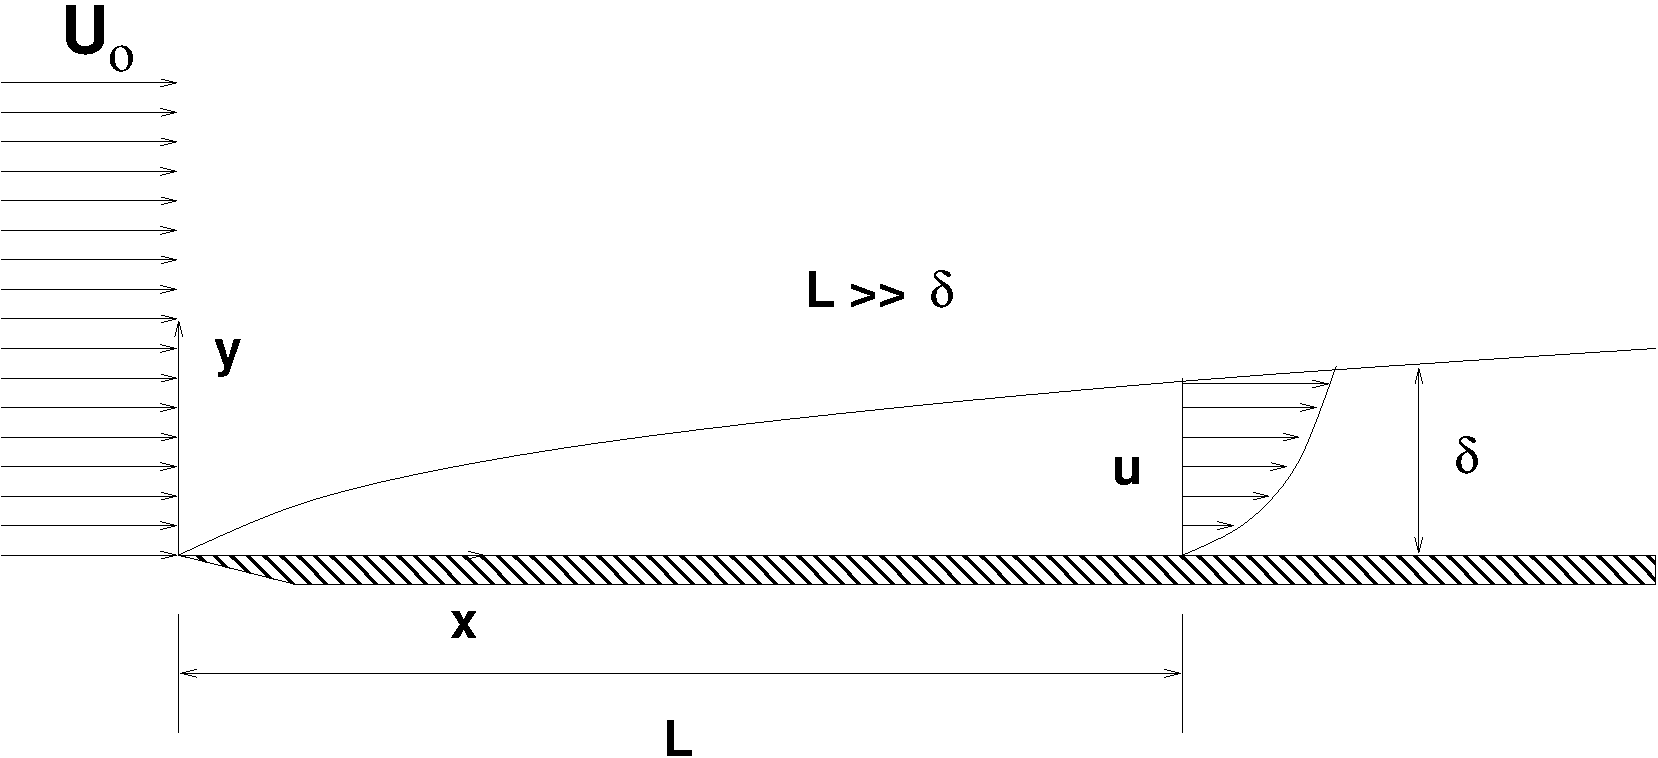
\includegraphics[width=0.85\textwidth]{./figuras/camada-limite.pdf}
\caption{Camada limite em uma placa plana}
\label{fig:blayer}
\end{figure}

Este tipo de análise pode ser levada mais adiante. Um problema mais simples é o escoamento em uma placa plana que pode ser visto na figura \ref{fig:blayer} onde a vista foi explodida na direção y de modo que $\delta_* = \delta/L \ll 1$ onde ao invés do diâmetro $D$ da esfera, utiliza-se como escala o comprimento da placa $L$. Repetindo o que se foi feito nas seções anteriores, as escalas $U_0$ e $L$ são utilizadas para se definir $U_*$ e $x_*$. Mas no caso da direção y, outra escala é empregada: $y_* = y / \delta$ onde $\delta$ é a espessura da camada limite ainda não conhecida. Assim, as equações de Navier-Stokes, em regime permanente, tomam a seguinte forma:
\begin{align}
 u_*\frac{\partial u_*}{\partial x_*} + v_*\frac{\partial u_*}{\partial y_*} &= 
-\frac{\partial p_*}{\partial x_*} + \frac{1}{Re} \left( \frac{\partial^2 u_*}{\partial x_*^2} + \frac{\partial^2 u_*}{\partial y_*^2}\right) \\
 u_*\frac{\partial v_*}{\partial x_*} + v_*\frac{\partial v_*}{\partial y_*} &= 
-\frac{\partial p_*}{\partial y_*} + \frac{1}{Re} \left( \frac{\partial^2 v_*}{\partial x_*^2} + \frac{\partial^2 v_*}{\partial y_*^2}\right) \\
\frac{\partial u_*}{\partial x_*} &+ \frac{\partial v_*}{\partial y_*} = 0\\
\end{align}

A partir das principais escalas do problema, pode-se obter uma estimativa da ordem de grandeza de cada termo das equações anteriores. Para a equação de Navier-Stokes na direção $x$ temos:
\[
\begin{matrix}
 u_*&\frac{\partial u_*}{\partial x_*} + &v_*&\frac{\partial u_*}{\partial y_*} =& 
-\frac{\partial p_*}{\partial x_*} + &\frac{1}{Re} &\left( \frac{\partial^2 u_*}{\partial x_*^2}\right. +& \left.\frac{\partial^2 u_*}{\partial y_*^2}\right) \\
1 & \frac{1}{1} & \delta^* & \frac{1}{\delta^*} & ? & ? & 1 & \frac{1}{\delta_*^2} \\
\end{matrix}
\]
nesta equação o único termo que pode ser desprezado é o termo difusivo em x $\frac{\partial^2 u_*}{\partial x_*^2}$. Pode não parecer muito mas isto simplifica o problema de uma maneira fundamental. A equação diferencial que originalmente era elíptica agora se torna parabólica! Mas ainda não temos uma estimativa para $Re$. Lembrando que na camada limite este termo é importante, é preciso que este termo tenha uma ordem de grandeza pelo menos igual ao resto da equação:
\[
\frac{1}{Re} \frac{\partial^2 u_*}{\partial x_*^2} \sim 1 \qrq Re \sim \frac{1}{\delta_*^2}
\]
(novamente, este é a maior estimativa nesta equação mas em geral os outros termos podem se cancelar).

Já a equação na direção $y$ muda significativamente:

\[
\begin{matrix}
u_*&\frac{\partial v_*}{\partial x_*} + &v_*&\frac{\partial v_*}{\partial y_*} =& 
-\frac{\partial p_*}{\partial y_*} + &\frac{1}{Re} &\left( \frac{\partial^2 v_*}{\partial x_*^2}\right. +& \left.\frac{\partial^2 v_*}{\partial y_*^2}\right) \\
 1 & \delta_* & \delta_* & 1 & ? & \delta_*^2 & \delta_* & \frac{1}{\delta_*} \\
\end{matrix}
\]
de modo que 
\[
\frac{\partial p_*}{\partial y_*} = \bigO{\delta_*} \approx 0
\]
isto quer dizer que a pressão não varia ao longo da espessura da camada limite, ou seja, a pressão em uma dada posição $x$ assume o valor da pressão na região fora da camada limite. Assim, nesta aproximação, a pressão é mais um parâmetro externo, um tipo de condição de contorno:
\[
p_* = p_*(x)
\]
Esta equação será resolvida para o caso mais simples, quando não há gradiante de pressão.

\subsubsection{A solução de Blasius}

Existe um sutileza na análise da camada limite apresentada até agora. Será que a escala $\delta$ é realmente apropriada? Ao final do comprimento $L$, esta análise é consistente. Mas e para $x < L$? Se o escoamento tem algo a ver com o que se vê na figura \ref{fig:blayer} claramente $\delta = \delta(x)$, ou seja, $\delta$ é uma escala local que varia ao longo do escoamento. É aí que o fato da equação diferencial ser parabólica se torna importante. A escoamento só depende do que veio antes, sua história. 

Para usar uma notação mais usual encontrada na literatura pode-se definir:
\[
y_* = \frac{y}{\delta} = \frac{y}{\delta(x)} = \eta
\]
Assim o campo de velocidade é dado por
\[
\frac{u}{U_0} = g\left[\frac{y}{\delta(x)}\right] = g(\eta)
\]
nesta equação está se admitindo uma hipótese importante: o perfil de velocidade não muda com $x$, exceto por um fator de escala. Está se admitindo que existe autosemelhança. É mais simples trabalhar com a função corrente
\[
\psi = U_0 \delta(x) f(\eta) \qquad \frac{u}{U_0} = \frac{\partial\psi}{\partial y}=f'(\eta)=g(\eta) \qquad \frac{v}{U_0} =-\frac{\partial\psi}{\partial x} = \frac{d\delta}{dx}\left(\eta f' - f\right)
\]
Falta, agora, determinar a função $\delta(x)$ a ser utilizada nesta equação. Uma estimativa para esta espessura foi obtida na equação \ref{eq:delta}. Definindo 
\begin{equation}
  \frac{\delta(x)}{x} = \sqrt{\frac{2}{Re_x}} \qrq \delta(x) = \sqrt{\frac{\nu x}{U_0}}
  \label{eq:delta2}
\end{equation}
onde o fator (2) é convencional e aparece em boa parte da literatura mas de maneira nenhuma necessário - estamos falando em ordem de grandeza afinal. Estas relações podem ser substituídas nas equações anteriores para se chegar à equação diferencial final.

Por outro lado, mesmo sem conhecer uma estimativa para $\delta(x)$, a relação anterior pode ser obtida postulando autosemelhança. Substituindo as expressões com $\delta(x)$ na equação da camada limite, lembrando que 
\[
\frac{\partial u}{\partial x} = -U_0\eta f'' \frac{d\delta}{dx}, 
\quad \frac{\partial u}{\partial y} = \frac{U_0 \cdot f''}{\delta}, \quad \frac{U_0 \cdot f'''}{\delta^2}
\]
chega-se à seguinte equação:
\[
\frac{U_0^2}{\delta}\frac{d\delta}{dx} ff'' + \frac{\nu U_0}{\delta^2}f''' = 0
\]
Para que a solução seja auto-semelhante, a equação acima não pode depender diretamente de $x$ de modo que
\[
\frac{U_0^2}{\delta}\frac{d\delta}{dx} \propto \frac{\nu U_0}{\delta^2} \qrq \delta^2 \propto \frac{\nu x}{U_0} + const \qrq \delta = \sqrt{\frac{2 \nu x}{U_0}}
\]
onde o fator (2) na última expressão é utilizado por uma questão de conveniência. Esta é, como esperado, a mesma expressão para $\delta(x)$ obtida utilizando a escala da equação \ref{eq:delta2}. Assim, chegamos à equação de Blasius:
\[
ff'' + f''' = 0
\]
com as seguintes condições de contorno:
\[
f = f' = 0 \quad\text{em}\quad \eta = 0
\]
\[
f' \lra 1 \quad\text{quando}\quad \eta\lra\infty
\]
É interessante notar que a expressão de $\delta$ nas equações acima é, fora o fator numérico $\sqrt{2}$ o mesmo que obtivemos na equação \ref{eq:delta}:
\[
\frac{\delta}{x} = \frac{1}{x}\cdot \sqrt{\frac{2 \nu x}{U_0}} = \sqrt{\frac{2}{Re_x}}
\]
onde ao invés de $Re$ (definido com a escala de comprimento $L$) temos $Re_x$ (definido com a escala de comprimento $x$). Aqui se pode perceber um problema: o que acontece quando $x\lra 0$? Existe uma singularidade nesta situação  mas isto é consistente com as hipóteses básicas da teoria da camada limite onde existem duas escalas muito distintas. Quando $x$ é muito pequeno, esta hipótese deixa de ser válida e a equação da camada limite não representa bem o fenômeno e deve ser descartada. Nesta região, outro modelo deve ser utilizado.



\subsection{Será que o problema da esfera já está resolvido?}

Diferentes aspectos do escoamento ao redor de uma esfera foram considerados mas a lista considerável de outros fatores podem influenciar no fenômeno que podem, eventualmente, ser importantes. Também não se pode esquecer que mesmo um fenômeno complexo como o escoamento ao redor de uma esfera já é um simplificação considerável. 

Nenhuma esfera é uma esfera de verdade. Como entra a rugosidade? A crise do arrasto mostra que um parâmetro pequeno (rugosidade) pode ter um efeito drástico no escoamento em algumas circunstâncias. Nenhuma esfera está isolada: sempre existem paredes que podem influenciar mais ou menos o escoamento. Mesmo quando o modelo simplificado inicial não é o suficiente, pode servir como uma referência. Além disso sempre existe alguma compressibilidade que à medida que a velocidade aumenta vai ter uma importância maior. Não estamos nem falando de outros fenômenos como transferência de calor ou efeitos moleculares.


\section{Semelhança}

Uma situação comum é realizar testes com modelos em escala reduzida. Mas, agora, qual a relação entre as grandezas no modelo em escala com o protótipo? Na metodologia apresentada até este ponto isto é simples: enquanto as escalas forem definidas de maneira consistente, as equações adimensionais (variáveis e operadores com sub-índice ``$*$'') são invariantes enquanto os parâmetros adimensionais forem os mesmos. No caso do escoamento ao redor de uma esfera, é necessário que a seguinte igualdade seja satisfeita:
\[
Re_m = Re_p
\]
onde $m$ se refere a modelo e $p$ se refere a protótipo. Se $\lambda_D = D_m/D_p$, $\lambda_U = U_m/U_p$ e $\lambda_\nu = \nu_m/\nu_p$, a igualdade do número de Reynolds necessita da seguinte relação entre escalas:
\[
\lambda_U\cdot\lambda_D = \lambda_\nu
\]



Se esta esfera estiver em uma base elástica, outros parâmetros como a velocidade reduzida $V_R = U_0/(\omega_N\cdot D)$  e a razão de massa $\rho D^3/m$ (as escalas de velocidade, comprimento e viscosidade respectivamente) devem ser iguais no modelo e no protótipo. 

Se estes parâmetros e as condições de contorno forem as mesmas no modelo e no protótipo, as mesmas equações são satisfeitas e têm, portanto a mesma solução. Isto é válido enquanto o modelo matemático utilizado for válido. Mas cuidado, muitas vezes efeitos de escala aparecem como por exemplo rugosidade. Se o modelo e o protótipo tiver o mesmo tipo de acabamento com mesma rugosidade, o modelo terá efetivamente uma rugosidade maior e isto pode ser importante. Outra dificuldade comum são folgas pequenas que são difíceis de serem reproduzidas em um modelo em escala reduzida.
